%% ============================================================================
%%  QUANTUM COMPUTING — COURSE PROJECT REPORT TEMPLATE
%%  ELEC/PHYS 450/550 · Spring 2026
%% ============================================================================
\documentclass[12pt, a4paper]{article}

% ── Packages ─────────────────────────────────────────────────────────────────
\usepackage[utf8]{inputenc}
\usepackage[T1]{fontenc}
\usepackage[margin=1in]{geometry}
\usepackage{graphicx}
\usepackage{amsmath, amssymb}
\usepackage{booktabs}
\usepackage{array}
\usepackage{tabularx}
\usepackage{xcolor}
\usepackage{colortbl}
\usepackage{hyperref}
\usepackage{fancyhdr}
\usepackage{titlesec}
\usepackage{setspace}
\usepackage{enumitem}
\usepackage{caption}
\usepackage{fancyhdr}
\usepackage{float}
\usepackage{braket}           % Dirac notation: \bra, \ket, \braket
\usepackage{qcircuit}         % Quantum circuit diagrams (optional)
\usepackage{listings}         % Code listings

% ── Colors ───────────────────────────────────────────────────────────────────
\definecolor{darkblue}{HTML}{000000}
\definecolor{accentblue}{HTML}{000000}
\definecolor{lightblue}{HTML}{E8F0F8}
\definecolor{darkred}{HTML}{8B0000}
\definecolor{placeholder}{HTML}{999999}
\definecolor{edityellow}{HTML}{FFE800}

% ── Hyperref Setup ───────────────────────────────────────────────────────────
\hypersetup{
    colorlinks=true,
    linkcolor=darkblue,
    citecolor=accentblue,
    urlcolor=accentblue,
}

% ── Section Formatting ───────────────────────────────────────────────────────
\titleformat{\section}
    {\Large\bfseries\color{darkblue}}
    {\thesection.}{0.5em}{}
    [\vspace{2pt}\textcolor{accentblue}{\titlerule[1.5pt]}]

\titleformat{\subsection}
    {\large\bfseries\color{accentblue}}
    {\thesubsection}{0.5em}{}

\titleformat{\subsubsection}
    {\normalsize\bfseries\color{darkblue!80}}
    {\thesubsubsection}{0.5em}{}

% ── Page style ────────────────────────────────────────────
\pagestyle{fancy}
\fancyhf{}
\IfFileExists{ku_logo.jpg}{\fancyhead[L]{
\includegraphics[height=20pt]{ku_logo.jpg}}}{\fancyhead[L]{}}%
\fancyhead[C]{\footnotesize ELEC/PHYS 450/550 QUANTUM COMPUTING}%
\fancyhead[R]{\footnotesize SPRING 2026}%
\fancyfoot[C]{\thepage}%
\renewcommand{\headrulewidth}{0.4pt}
\renewcommand{\footrulewidth}{0pt}
\setlength{\headheight}{25pt}

% ── Code Listing Style ──────────────────────────────────────────────────────
\lstset{
    basicstyle=\ttfamily\small,
    backgroundcolor=\color{lightblue},
    frame=single,
    rulecolor=\color{accentblue!50},
    breaklines=true,
    numbers=left,
    numberstyle=\tiny\color{placeholder},
    keywordstyle=\color{darkblue}\bfseries,
    commentstyle=\color{placeholder}\itshape,
    stringstyle=\color{accentblue},
    tabsize=4,
}

% ── Placeholder Command ─────────────────────────────────────────────────────
\newcommand{\placeholder}[1]{\textit{\textcolor{placeholder}{#1}}}
\newcommand{\changefield}[1]{\colorbox{edityellow}{\textit{\textcolor{placeholder}{#1}}}}
\newcommand{\changefieldblock}[1]{\colorbox{edityellow}{\parbox{\dimexpr\linewidth-2\fboxsep\relax}{\textit{\textcolor{placeholder}{#1}}}}}

% ── Custom Table Environments ────────────────────────────────────────────────
\newcolumntype{L}[1]{>{\raggedright\arraybackslash}p{#1}}
\newcolumntype{C}[1]{>{\centering\arraybackslash}p{#1}}

% ── Caption Positioning ─────────────────────────────────────────────────────
\captionsetup[table]{position=top,skip=4pt}

% ══════════════════════════════════════════════════════════════════════════════
\begin{document}
\pagenumbering{roman}
\thispagestyle{fancy}
% ═══════════════════════════ COVER PAGE ═══════════════════════════════════════
\begin{titlepage}
    \centering
    \vspace*{2cm}

    
\includegraphics[width=0.48\textwidth]{ku_logo.png}\\[18pt]

    

    {\large\textbf{\textcolor{black}{ELEC/PHYS 450/550}}}\\[6pt]
    {\Large\textbf{\textcolor{black}{QUANTUM COMPUTING}}}\\[6pt]
    {\LARGE\textbf{\textcolor{black}{COURSE PROJECT REPORT}}}\\[30pt]
    {\large\textcolor{black}{SPRING 2026}}\\[20pt]

    \textcolor{black}{\rule{0.7\textwidth}{1.5pt}}\\[16pt]
  {\Large\textbf{Quantum Reinforcement Learning for Grid World Navigation: A Comparative Analysis}}\\[16pt]
    \textcolor{black}{\rule{0.7\textwidth}{1.5pt}}\\[40pt]

    {\large\textbf{Prepared by}}\\[8pt]
    {\large Barış Cem Bakay}\\[4pt]
    {\large Student ID: 0082990}\\[30pt]

    {\large May 31, 2026}\\[60pt]

    \vfill

    \vspace{1cm}

\end{titlepage}
\setcounter{page}{2}

% ═══════════════════════ TABLE OF CONTENTS ════════════════════════════════════
\newpage
\tableofcontents
\newpage

% ══════════════════════════════════════════════════════════════════════════════
%  1. ABSTRACT
% ══════════════════════════════════════════════════════════════════════════════
\section{Abstract}

This project presents a comparative analysis between Classical Deep Q-Networks (DQN) and Quantum Variational Quantum Circuits (VQC) applied to a discrete Grid World navigation task. We model the navigation task as a Markov Decision Process in a custom Gymnasium environment. For the classical baseline, we implement a multi-layer feedforward neural network in PyTorch containing 4,612 trainable parameters. For the quantum policy network, we construct a 4-qubit Variational Quantum Circuit in Qiskit, utilizing Angle Encoding for state representation and the RealAmplitudes ansatz for the trainable policy, totaling 36 parameters (16 quantum rotation angles and 20 classical post-processing weights). Both agents are trained and evaluated on 3x3 and 4x4 grids. Our results show that both classical and quantum reinforcement learning agents successfully converge to optimal navigation trajectories, achieving perfect rewards of $+0.88$ on 3x3 grids and $+0.72$ on 4x4 grids. We verify the coherence of the quantum policy network via exact state tomography, obtaining a state purity of $1.0$ and a Von Neumann entropy of $0.0$, indicating noise-free, pure coherent superposition. Although the quantum agent demonstrates a 99.2\% reduction in parameter count and high scaling efficiency, it exhibits significant classical simulation overhead due to gradient calculation via the Parameter-Shift rule. We discuss how native QPU execution or advanced quantum differentiation methods can overcome this computational bottleneck.


\newpage

% ══════════════════════════════════════════════════════════════════════════════
%  2. INTRODUCTION
% ══════════════════════════════════════════════════════════════════════════════
\section{Introduction}

\subsection{Background and Motivation}

Reinforcement Learning (RL) has emerged as a cornerstone for sequential decision-making, with applications spanning robotics, autonomous navigation, and resource allocation \cite{sutton2018}. Traditional Deep Reinforcement Learning (DRL) relies on deep neural networks (DNNs) as function approximators to estimate action values or policies \cite{mnih2015}. Despite their success, DNNs are highly over-parameterized, requiring thousands to millions of weights, which demands substantial memory and training data. 

With the advent of Noisy Intermediate-Scale Quantum (NISQ) computing \cite{preskill2018}, Quantum Machine Learning (QML) has emerged as a promising alternative \cite{biamonte2017}. Variational Quantum Circuits (VQCs) are particularly attractive for hybrid quantum-classical algorithms \cite{cerezo2021}. VQCs utilize parameterized quantum gates that can be trained using classical optimizers. In this context, Quantum Reinforcement Learning (QRL) seeks to replace classical neural networks with VQCs, potentially offering extreme parameter efficiency and leveraging quantum entanglement and superposition. This project explores the feasibility of QRL on a discrete Grid World navigation task, comparing its convergence behavior, parameter scaling, and simulation complexity against a classical DQN baseline.



\subsection{Problem Definition}

We model the Grid World navigation task as a discrete Markov Decision Process (MDP) $(\mathcal{S}, \mathcal{A}, \mathcal{P}, \mathcal{R}, \gamma)$. The agent starts at state $(0,0)$ and must find the shortest path to the goal state $(N-1, N-1)$ while avoiding static obstacles. We define the problem elements in Table \ref{tab:problem_definition}.


\begin{table}[H]
    \centering
    \caption{Problem definition elements.}
    \label{tab:problem_definition}
    \renewcommand{\arraystretch}{1.3}
    \begin{tabularx}{\textwidth}{|L{4.0cm}|X|}
        \hline
        \rowcolor{darkred!90}
        \textcolor{white}{\textbf{Element}} & \textcolor{white}{\textbf{Description}} \\
        \hline
        \rowcolor{darkred!20}
        Variables & Agent state coordinate vector $s = (x, y) \in [0, N-1]^2$; action $a \in \{0, 1, 2, 3\}$ (representing Up, Down, Left, Right); reward $r \in \{+1.0, -1.0, -0.04\}$ representing Goal state reach, Obstacle collision, and transition step penalty respectively. \\
        \hline
        Governing Equations & Bellman Optimality Equation:
        \[ Q^*(s, a) = R(s, a) + \gamma \max_{a'} Q^*(s', a') \]
        Loss function for Q-learning network with parameters $\theta$ and target network parameters $\theta^-$:
        \[ L(\theta) = \mathbb{E} \left[ \left( r + \gamma \max_{a'} Q(s', a'; \theta^-) - Q(s, a; \theta) \right)^2 \right] \] \\
        \hline
        \rowcolor{darkred!20}
        Constraints & Grid boundaries: $0 \le x, y < N$. Obstacle state $(1, 1)$ terminates the episode with reward $-1.0$. Step limit of 50 steps per episode. \\
        \hline
        Target Metrics & Path optimality: total reward of $+0.88$ (3-step path) for 3x3 grid, $+0.72$ (7-step path) for 4x4 grid. Policy network state purity $\gamma = \text{Tr}(\rho^2) = 1.0$ and Von Neumann entropy $S = 0.0$ under unitary simulation. \\
        \hline
        \rowcolor{darkred!20}
        Input/Output & \raggedright Input: Cartesian state coordinates $(x, y) \in \mathbb{R}^2$. \newline Output: Action-value vector $\vec{Q}(s) = [Q(s, 0), Q(s, 1), Q(s, 2), Q(s, 3)]^T \in \mathbb{R}^4$. \tabularnewline
        \hline
    \end{tabularx}
\end{table}

\begin{figure}[H]
    \centering
    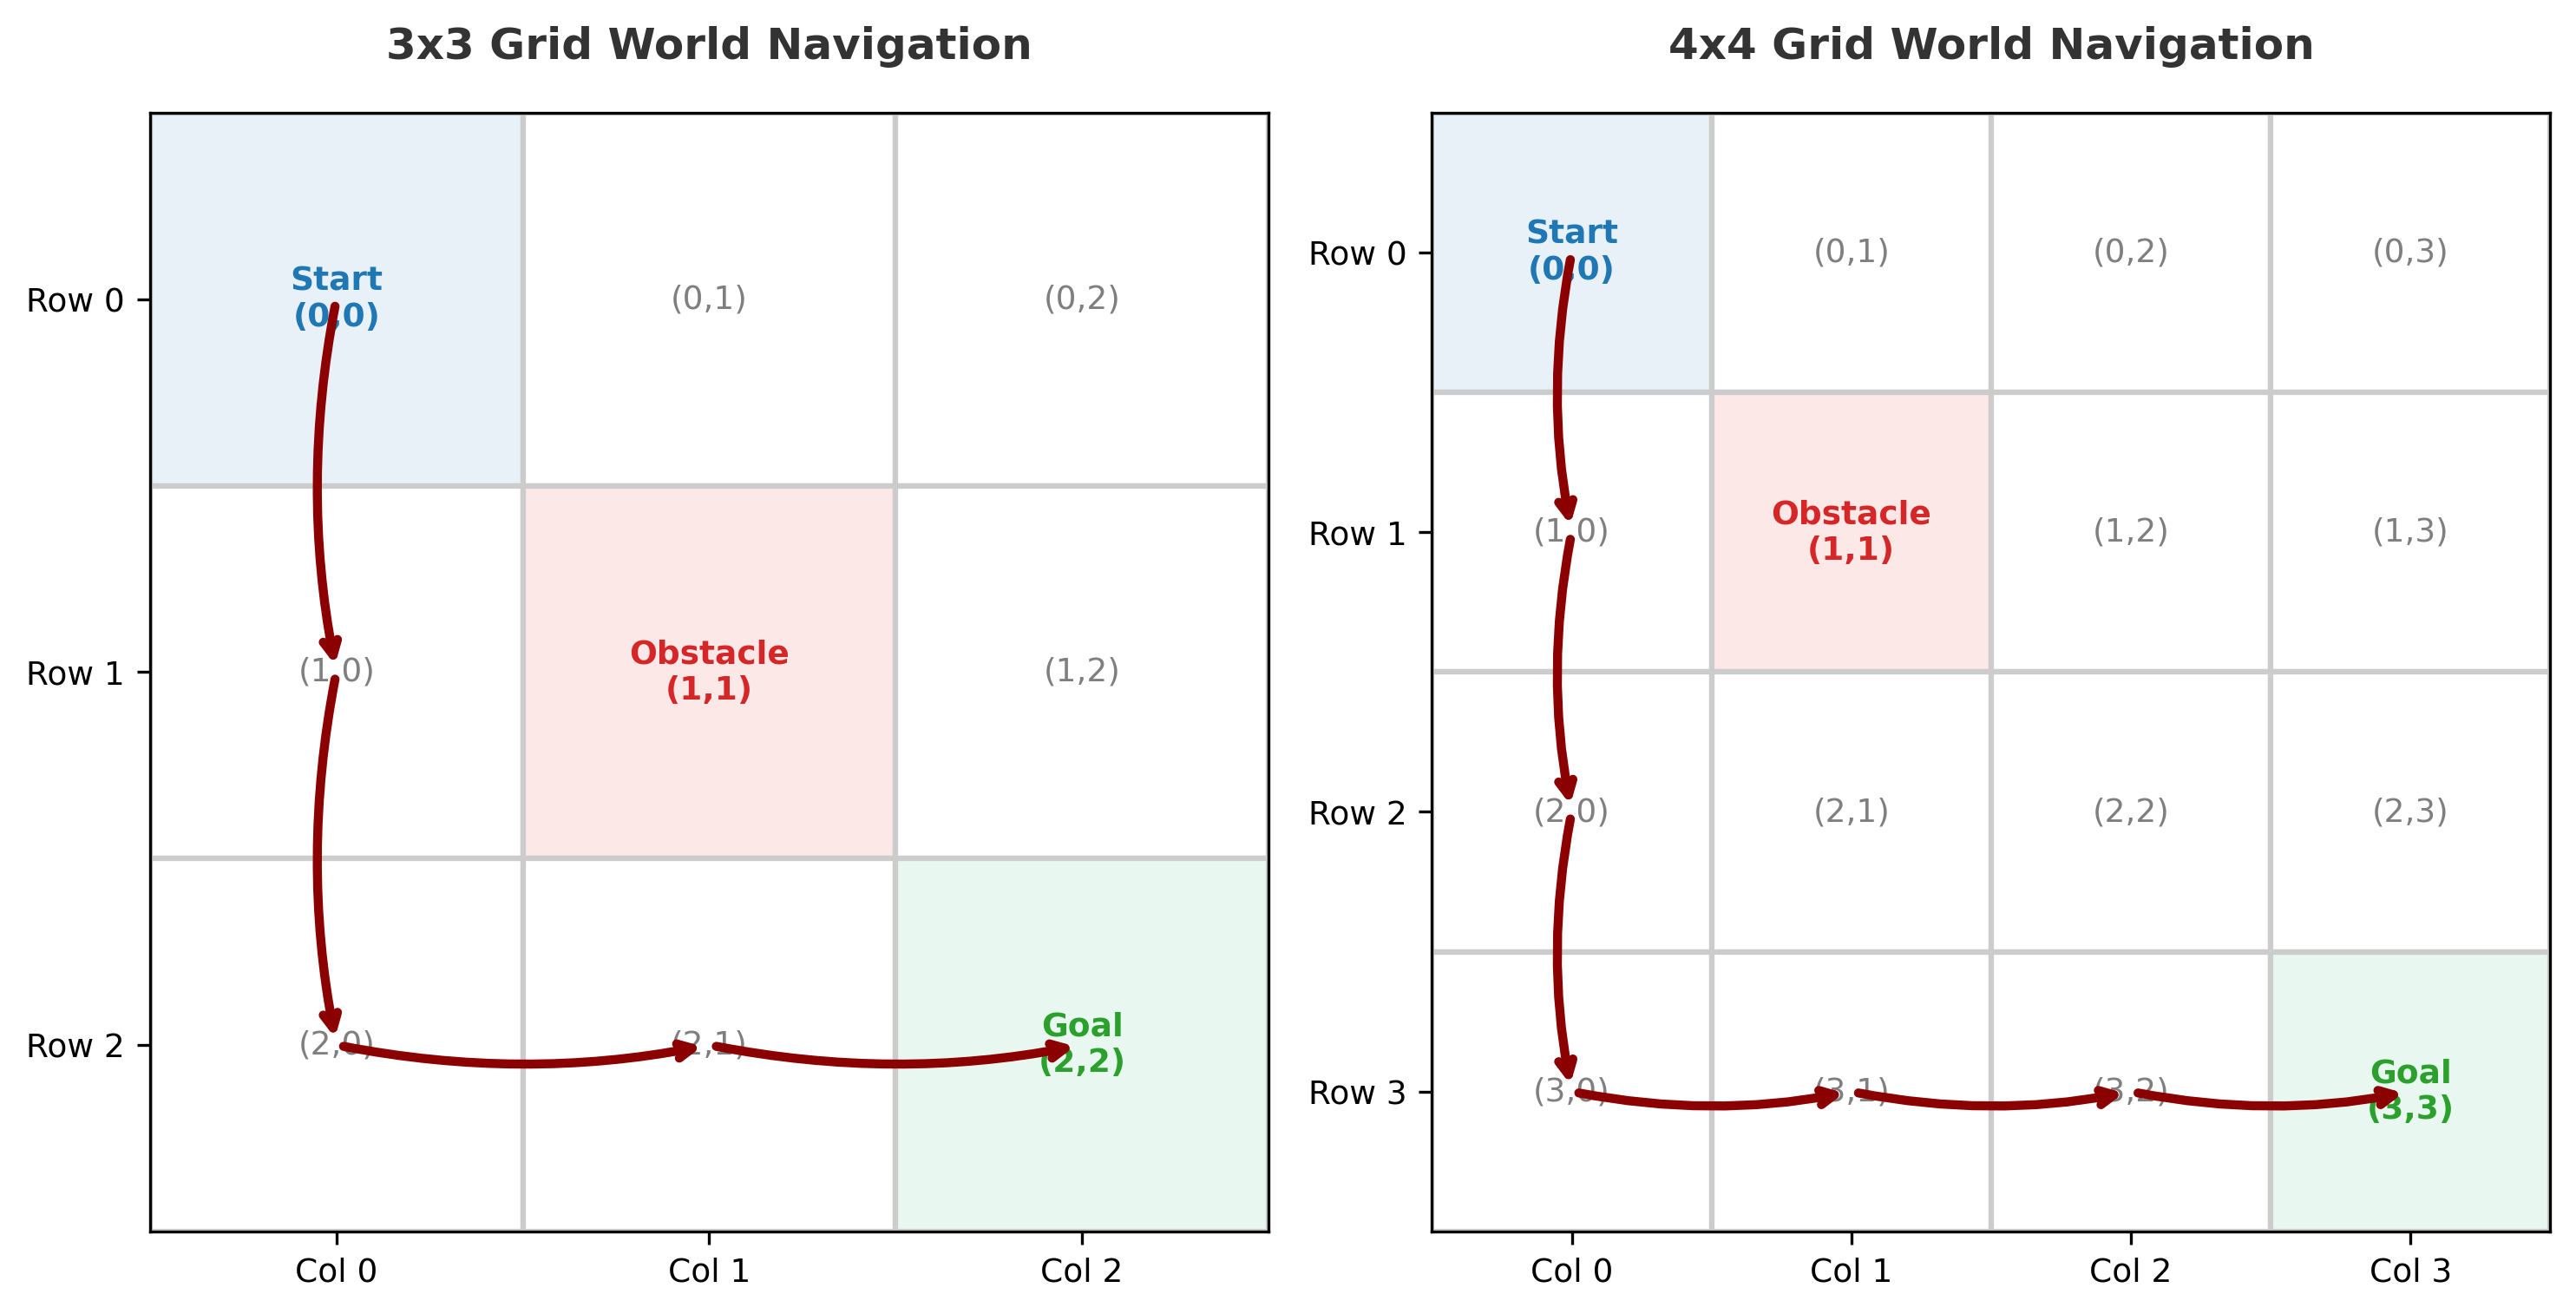
\includegraphics[width=0.85\textwidth]{../results/grid_world_visualization.png}
    \caption{Grid World environment configurations showing the state representation, coordinate system, and optimal path navigation for (a) the $3\times3$ grid environment and (b) the $4\times4$ grid environment.}
    \label{fig:grid_world_visualization}
\end{figure}

\subsection{Hypothesis}

We hypothesize that the Variational Quantum Circuit (VQC) policy network can successfully learn the optimal navigation policy in the Grid World environment. Specifically, we expect the quantum approach to achieve comparable navigation accuracy to the classical DQN baseline while utilizing significantly fewer trainable parameters (an order of magnitude reduction). However, due to the classical simulation of quantum circuits and gradient calculations using the Parameter-Shift rule, we expect the quantum agent to exhibit higher training time compared to the classical baseline.

\subsection{Literature Review}

The integration of deep learning with reinforcement learning was pioneered by Mnih et al. \cite{mnih2015}, demonstrating control on Atari games using Deep Q-Networks. However, the parameter cost of these models is substantial. In parallel, Biamonte et al. \cite{biamonte2017} outlined the potential of quantum computing to enhance machine learning tasks, suggesting speedups in representation and optimization. 

For reinforcement learning, Chen et al. \cite{chen2020} introduced Variational Quantum Circuits for deep Q-learning, demonstrating that VQCs can function as effective Q-value approximators. Jerbi et al. \cite{jerbi2021} investigated parametric quantum policies, proving that quantum policies can offer representational advantages in specific reinforcement learning tasks. Furthermore, Lockwood and Si \cite{lockwood2020} successfully applied VQCs to grid environments, demonstrating convergence on basic navigation tasks. Despite these promising results, the training stability and computational scaling of VQCs on classical simulators remain a challenge. This project builds on these works by performing a rigorous comparative scaling analysis (3x3 vs. 4x4) and verifying the coherence of the learned policy using exact quantum state tomography.

\newpage

% ══════════════════════════════════════════════════════════════════════════════
%  3. METHODOLOGY
% ══════════════════════════════════════════════════════════════════════════════
\section{Methodology}

\subsection{Classical Algorithm}

\subsubsection{Algorithm Selection and Justification}

We choose the Deep Q-Network (DQN) algorithm \cite{mnih2015} as our classical baseline. DQN is a value-based reinforcement learning algorithm that uses a neural network to approximate the action-value function $Q(s, a)$. It is highly suitable for discrete state-action spaces. To stabilize training and break temporal correlations, DQN utilizes an experience replay buffer and a separate target network $\theta^-$ that is updated periodically. The theoretical time complexity per step is $\mathcal{O}(W)$ where $W$ is the number of weights in the network.

\subsubsection{Implementation Details}

The classical DQN is implemented in Python using PyTorch. The state vector $(x, y)$ is fed into a feedforward neural network consisting of:
\begin{itemize}
    \item Input layer: 2 neurons (representing coordinates $x, y$).
    \item Hidden layers: Two dense layers with 64 neurons each and ReLU activation functions.
    \item Output layer: 4 linear neurons representing Q-values for the actions \{Up, Down, Left, Right\}.
\end{itemize}
The network has a total of 4,612 trainable parameters. We use the Adam optimizer with a learning rate of $0.001$, Mean Squared Error (MSE) loss, a replay buffer of capacity 5,000, batch size of 64, and an epsilon-greedy exploration strategy decaying from $1.0$ to $0.01$ at a rate of $0.995$ per episode.

\begin{figure}[H]
    \centering
    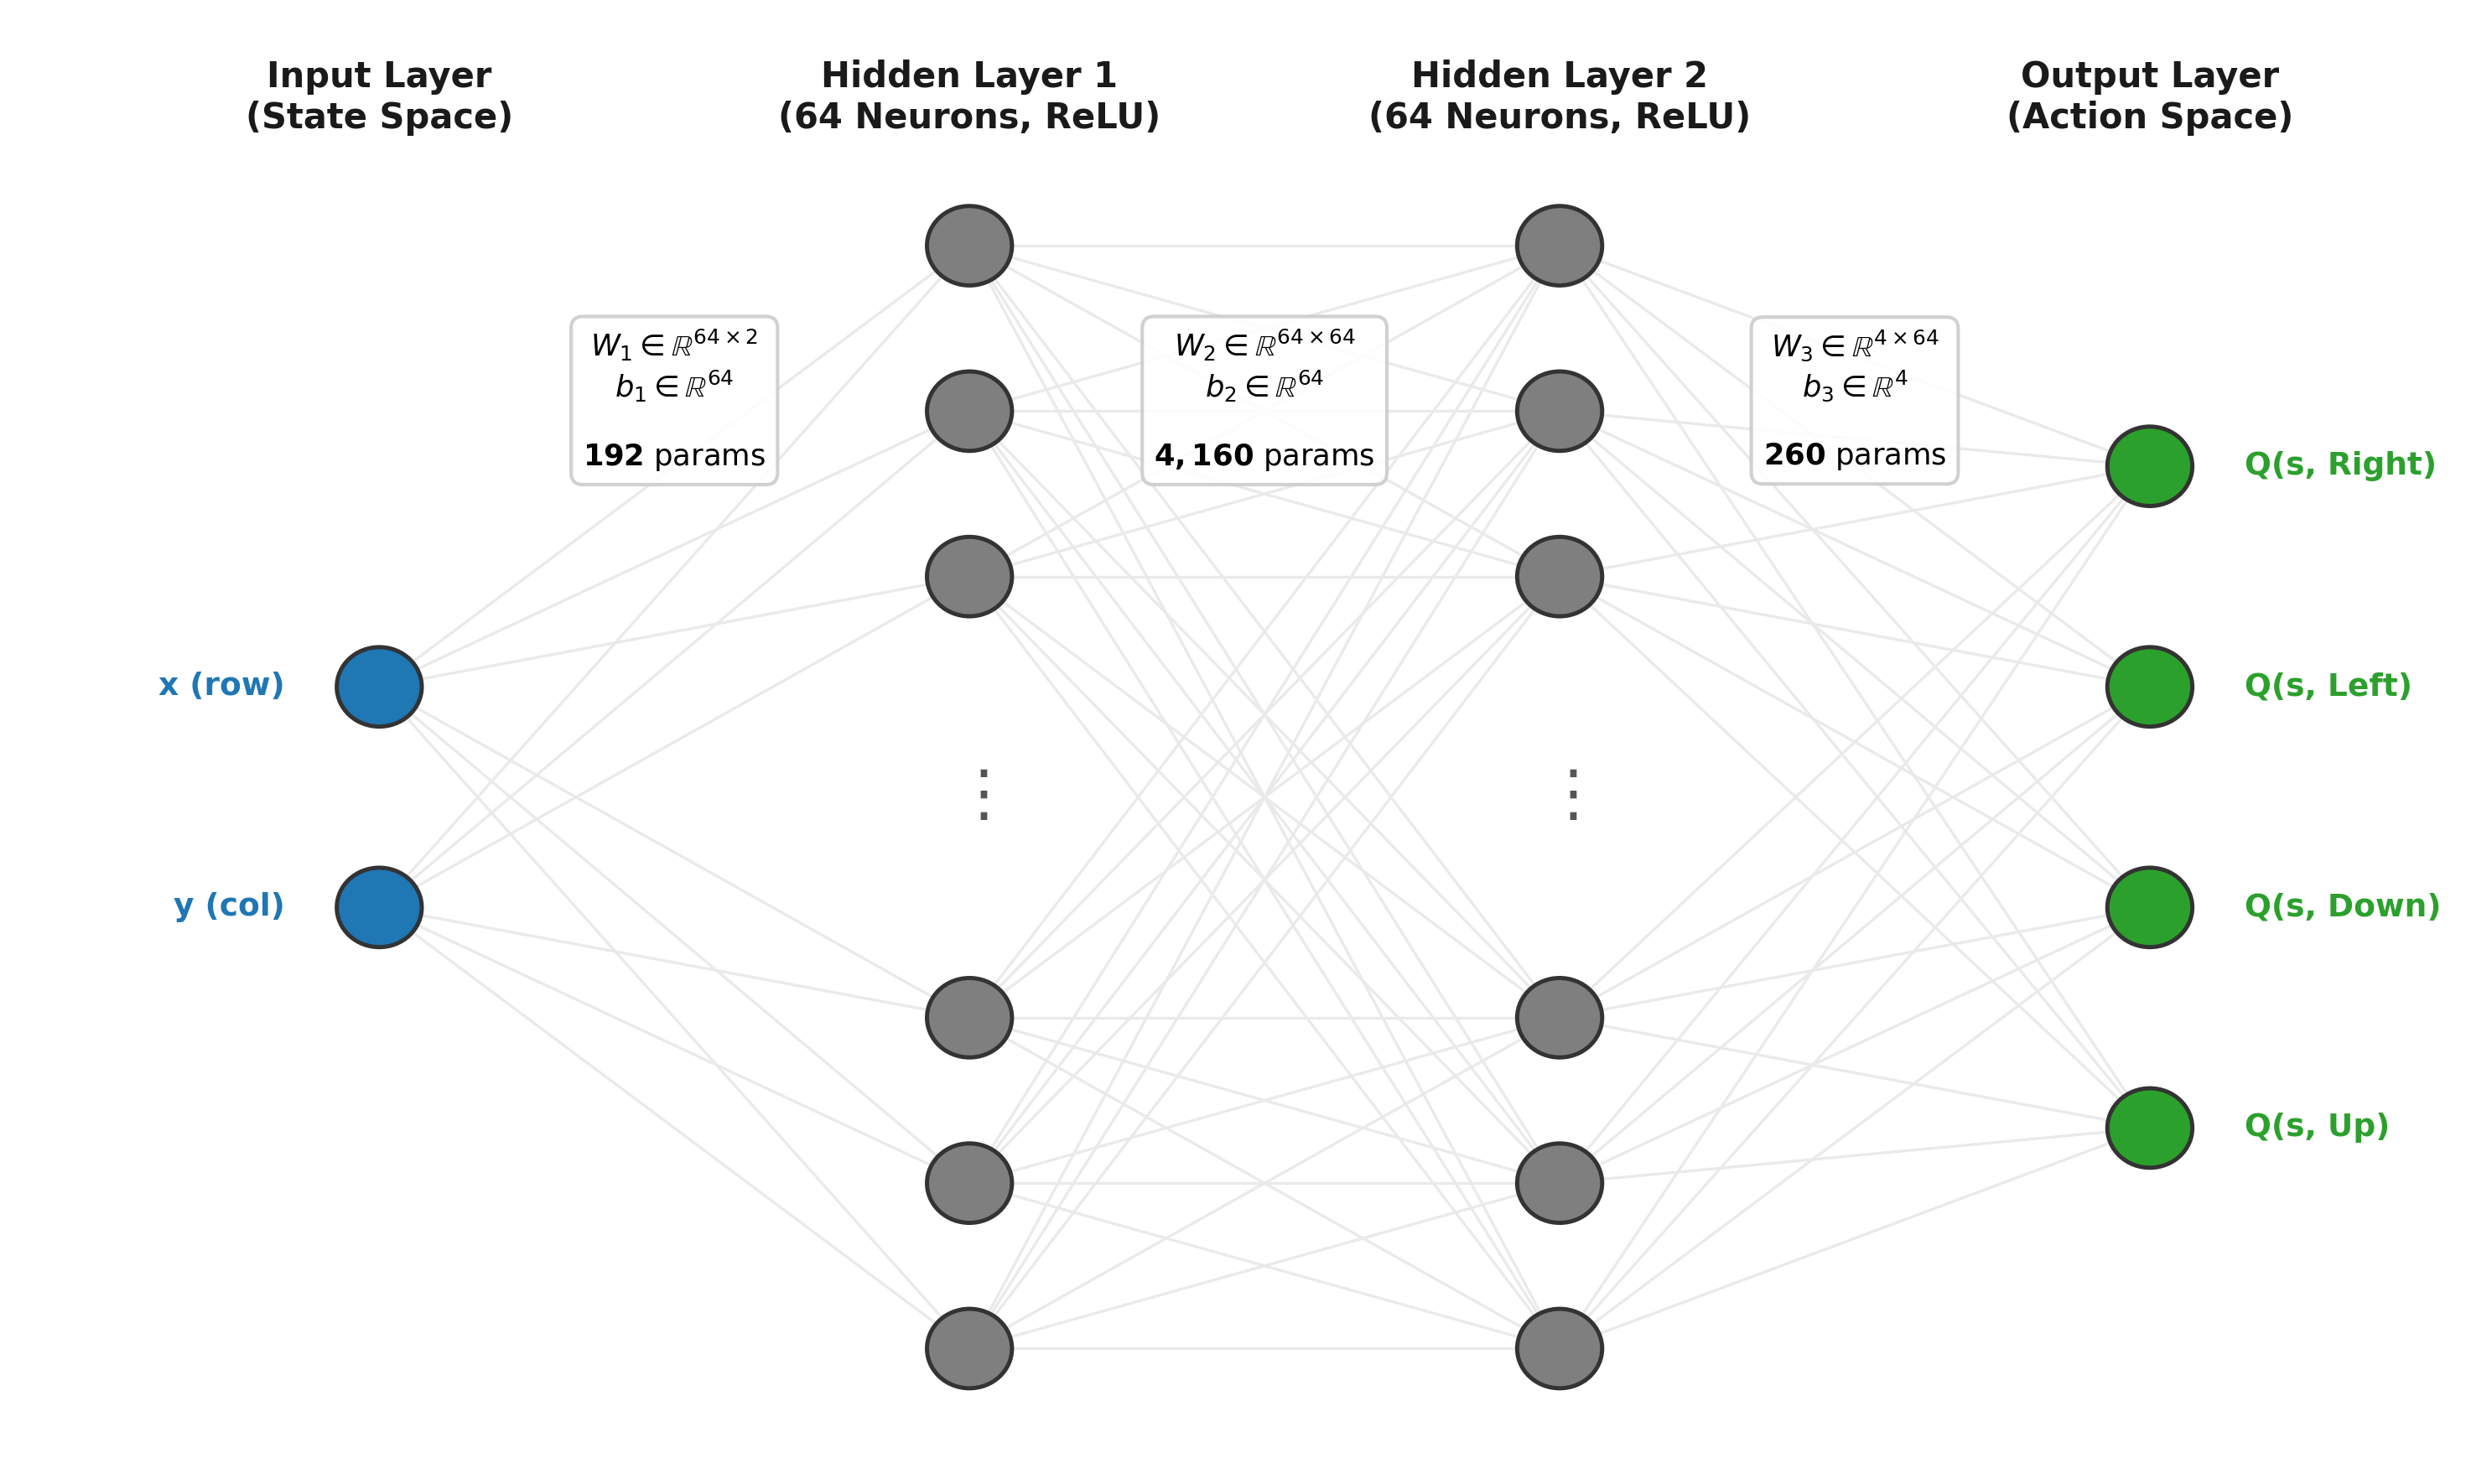
\includegraphics[width=0.85\textwidth]{../results/classical_dqn_agent.png}
    \caption{Classical Deep Q-Network (DQN) architecture detailing the input state vector, dense hidden layers with ReLU activations, and the action-value output layer.}
    \label{fig:classical_dqn_agent}
\end{figure}


% Example pseudocode block (students can replace or remove):
% \begin{lstlisting}[language=Python, caption={Classical algorithm pseudocode.}]
% def classical_solver(input_data):
%     # Initialize variables
%     # Main computation loop
%     # Return results
%     pass
% \end{lstlisting}

\subsubsection{Accuracy Verification}

We validate the correctness of our classical DQN by comparing the converged policy against the analytical shortest path solution. For a 3x3 grid, starting at $(0, 0)$, avoiding the obstacle at $(1, 1)$, and ending at $(2, 2)$, the shortest path is 3 steps, achieving a reward of $+0.88$ ($1.0 - 3 \times 0.04$). The classical agent converges rapidly to this value, showing that the implementation correctly solves the navigation problem.

\subsection{Quantum Algorithm}

\subsubsection{Algorithm Type and Justification}

We implement a hybrid Quantum-Classical Reinforcement Learning agent using a Variational Quantum Circuit (VQC) \cite{chen2020}. The VQC acts as the function approximator to estimate the action-value Q-values. This approach is highly suitable for NISQ devices as it requires very few qubits and shallow circuit depth, mitigating the effects of quantum noise and decoherence. The design choices are summarized in Table \ref{tab:quantum_design}.

\begin{table}[H]
    \centering
    \caption{Quantum algorithm design choices.}
    \label{tab:quantum_design}
    \renewcommand{\arraystretch}{1.3}
    \begin{tabularx}{\textwidth}{|L{5.5cm}|X|}
        \hline
        \rowcolor{darkred!90}
        \textcolor{white}{\textbf{Design Choice}} & \textcolor{white}{\textbf{Details}} \\
        \hline
        \rowcolor{darkred!20}
        Algorithm Type & Variational Quantum Circuit (VQC) DQN \\
        \hline
        Qubit Count & 4 qubits (one per discrete action: Up, Down, Left, Right) \\
        \hline
        \rowcolor{darkred!20}
        Circuit Depth & 13 gates (1 encoding layer + 3 reps of ansatz) \\
        \hline
        Ansatz / Oracle Design & Angle Encoding + `RealAmplitudes` with linear CNOT entanglement \\
        \hline
        \rowcolor{darkred!20}
        Classical Optimizer & Adam ($\text{lr} = 0.001$) with gradient clipping \\
        \hline
    \end{tabularx}
\end{table}

\subsubsection{Qiskit Implementation}

The quantum circuit is constructed using Qiskit. The state coordinates $(x, y)$ are normalized to $\theta \in [0, \pi]$ and encoded via $R_y(\theta)$ rotation gates applied to qubits 0, 1, 2, and 3 (with duplication to increase expressivity). This is followed by a `RealAmplitudes` ansatz with 3 repetition layers, where each layer contains single-qubit $R_y$ rotation gates and linear entangling CNOT gates between adjacent qubits.
The output Q-values are computed by evaluating the expectation values of the Pauli-Z operators on each qubit:
\[ Q(s, a_i) = \alpha_i \langle \psi(s, \theta) | \hat{Z}_i | \psi(s, \theta) \rangle + \beta_i \]
where $\alpha_i, \beta_i$ are trainable weights and biases of a classical output layer. This hybrid network is integrated into PyTorch using Qiskit Machine Learning's `TorchConnector` and trained using PyTorch's automatic differentiation with parameter-shift gradients.

\subsubsection{Quantum State Tomography}

To physically analyze the state of the quantum policy network during navigation, we perform exact quantum state tomography. We reconstruct the density matrix $\rho$ of the 4-qubit system at key grid coordinates: Start $(0,0)$, Obstacle Adjacent $(1,0)$, Near Goal $(2,1)$, and Goal $(2,2)$. We evaluate the state purity $\gamma = \text{Tr}(\rho^2)$ and Von Neumann entropy $S = -\text{Tr}(\rho \ln \rho)$ to verify the coherence of the quantum policy network.

\subsubsection{Quantum Circuit}

The hybrid Quantum-Classical policy network consists of three sequential processing stages: classical state normalization and encoding, variational quantum state rotation and entanglement, and classical linear scaling of output expectation values. 

\paragraph{State Normalization and Encoding}
The 2D state coordinates $s = (x, y) \in [0, N-1]^2$ are first classically normalized to the range $[0, \pi]$ using:
\begin{equation}
    \theta_x = \frac{\pi}{N-1} x, \quad \theta_y = \frac{\pi}{N-1} y
\end{equation}
These normalized angles are encoded into the 4-qubit quantum register via single-qubit $R_y$ rotations. To ensure that every qubit is initialized with state-dependent information, we duplicate the coordinates across the register such that:
\begin{equation}
    |\psi_{\text{enc}}(s)\rangle = R_y(\theta_x)^{\otimes 2} \otimes R_y(\theta_y)^{\otimes 2} |0000\rangle
\end{equation}
Specifically, $R_y(\theta_x)$ acts on qubits $q_0$ and $q_2$, while $R_y(\theta_y)$ acts on qubits $q_1$ and $q_3$. This encoding strategy expands the state-dependency across the entire register, enabling the subsequent entangling ansatz to model non-linear coordinate correlations.

\paragraph{Variational RealAmplitudes Ansatz}
Following a barrier that separates encoding from training, we apply the \texttt{RealAmplitudes} ansatz with $R = 3$ repetitions. The ansatz is parameterized by 16 trainable angles $\vec{\theta} \in \mathbb{R}^{16}$. 
\begin{enumerate}
    \item \textbf{Initial Rotation Layer (Repetition 0)}: Applies a parameterized $R_y(\theta_j)$ rotation to each qubit $q_j$ ($j \in \{0, 1, 2, 3\}$), introducing 4 parameters.
    \item \textbf{Entangling Layers}: In each of the 3 repetitions, linear entanglement is implemented using a cascade of three controlled-NOT (CNOT) gates between adjacent qubits: $C_{0\to1}$, $C_{1\to2}$, and $C_{2\to3}$.
    \item \textbf{Variational Rotation Layers}: Each CNOT cascade is followed by another layer of 4 parameterized $R_y(\theta_k)$ rotations.
\end{enumerate}
The total parameter count of the variational circuit is calculated as $N_{\text{qubits}} \times (R + 1) = 4 \times (3 + 1) = 16$ trainable angles. The output quantum state is expressed as $|\psi(s, \vec{\theta})\rangle = U(\vec{\theta}) |\psi_{\text{enc}}(s)\rangle$.

\paragraph{Expectation Values and Classical Scaling}
The final policy is extracted by measuring the expectation value of the Pauli-Z operator on each qubit:
\begin{equation}
    \langle Z_i \rangle = \langle \psi(s, \vec{\theta}) | \hat{Z}_i | \psi(s, \vec{\theta}) \rangle \in [-1, 1], \quad i \in \{0, 1, 2, 3\}
\end{equation}
To map these expectation values to discrete action Q-values, we pass them through a classical fully connected linear layer:
\begin{equation}
    Q(s, a_i) = \sum_{j=0}^{3} W_{ij} \langle Z_j \rangle + b_i
\end{equation}
where $W \in \mathbb{R}^{4 \times 4}$ represents the weight matrix and $b \in \mathbb{R}^4$ is the bias vector, introducing 20 classical parameters. The combined hybrid network contains $16$ quantum and $20$ classical parameters, for a total of $36$ trainable weights. 

\paragraph{Circuit Expressibility and Entanglement Capability}
The expressibility of a Variational Quantum Circuit (VQC) refers to its ability to generate states that are well-distributed across the Hilbert space, which directly determines its capacity to approximate complex non-linear functions \cite{sim2019}. In this design, expressibility and entangling power are maximized through two main strategies:
\begin{enumerate}
    \item \textbf{Input Duplication and Non-linear Feature Crosses}: 
    To map the 2D coordinate space $(x, y)$ to the 4-qubit register, we duplicate the coordinates so that qubits $q_0, q_2$ encode $x$ and $q_1, q_3$ encode $y$. The initial encoded state is:
    \begin{equation}
        |\psi_{\text{enc}}(s)\rangle = R_y(\theta_x)|0\rangle_{q_0} \otimes R_y(\theta_y)|0\rangle_{q_1} \otimes R_y(\theta_x)|0\rangle_{q_2} \otimes R_y(\theta_y)|0\rangle_{q_3}
    \end{equation}
    When CNOT gates are subsequently applied between adjacent qubits, they generate quantum entanglement. For example, applying a CNOT between $q_0$ and $q_1$ transforms the state as:
    \begin{align*}
        \text{CNOT}_{0\to1} \left(R_y(\theta_x)|0\rangle \otimes R_y(\theta_y)|0\rangle\right) &= \cos\left(\frac{\theta_x}{2}\right)\cos\left(\frac{\theta_y}{2}\right)|00\rangle + \cos\left(\frac{\theta_x}{2}\right)\sin\left(\frac{\theta_y}{2}\right)|01\rangle \\
        &+ \sin\left(\frac{\theta_x}{2}\right)\sin\left(\frac{\theta_y}{2}\right)|10\rangle + \sin\left(\frac{\theta_x}{2}\right)\cos\left(\frac{\theta_y}{2}\right)|11\rangle
    \end{align*}
    This creates product terms of coordinates (e.g., $\sin(\theta_x/2)\sin(\theta_y/2)$). These entangling cross-terms act as a non-linear feature mapping, enabling the circuit to represent complex boundary conditions, such as isolating the obstacle penalty at state $(1, 1)$.
    
    \item \textbf{Optimal Ansatz Depth ($R = 3$)}: 
    A higher repetition depth $R$ increases the circuit's expressibility by adding more variational parameters. However, in accordance with the barren plateau theorem \cite{mcclean2018}, random quantum circuits of large depth $D$ exhibit vanishing gradients, where the variance of the partial derivatives of local expectation values scales exponentially:
    \begin{equation}
        \text{Var}\left[\frac{\partial \langle Z_i \rangle}{\partial \theta_k}\right] \sim \mathcal{O}(2^{-n})
    \end{equation}
    where $n = 4$ is the number of qubits. By selecting $R=3$ repetitions, we provide exactly $16$ parameters. This is deep enough to cover the necessary state transitions (high expressibility), while remaining shallow enough to avoid barren plateaus and minimize gate decoherence on noisy intermediate-scale quantum devices.
\end{enumerate}

The detailed gate-level layout and the overall processing pipeline are illustrated in Figure \ref{fig:quantum_circuit} and Figure \ref{fig:quantum_vqc_agent}, respectively.

The structure of the quantum circuit is illustrated below:

\begin{figure}[H]
    \centering
    \resizebox{0.95\textwidth}{!}{
        \Qcircuit @C=0.8em @R=0.8em {
            \lstick{q_0: \ket{0}} & \gate{R_y(x)} & \qw & \barrier{3} & \qw & \gate{R_y(\theta_0)} & \ctrl{1} & \qw      & \qw      & \gate{R_y(\theta_4)} & \ctrl{1} & \qw      & \qw      & \gate{R_y(\theta_8)}  & \ctrl{1} & \qw      & \qw      & \gate{R_y(\theta_{12})} & \meter & \rstick{\langle Z_0 \rangle} \\
            \lstick{q_1: \ket{0}} & \gate{R_y(y)} & \qw & \qw         & \qw & \gate{R_y(\theta_1)} & \targ    & \ctrl{1} & \qw      & \gate{R_y(\theta_5)} & \targ    & \ctrl{1} & \qw      & \gate{R_y(\theta_9)}  & \targ    & \ctrl{1} & \qw      & \gate{R_y(\theta_{13})} & \meter & \rstick{\langle Z_1 \rangle} \\
            \lstick{q_2: \ket{0}} & \gate{R_y(x)} & \qw & \qw         & \qw & \gate{R_y(\theta_2)} & \qw      & \targ    & \ctrl{1} & \gate{R_y(\theta_6)} & \qw      & \targ    & \ctrl{1} & \gate{R_y(\theta_{10})} & \qw      & \targ    & \ctrl{1} & \gate{R_y(\theta_{14})} & \meter & \rstick{\langle Z_2 \rangle} \\
            \lstick{q_3: \ket{0}} & \gate{R_y(y)} & \qw & \qw         & \qw & \gate{R_y(\theta_3)} & \qw      & \qw      & \targ    & \gate{R_y(\theta_7)} & \qw      & \qw      & \targ    & \gate{R_y(\theta_{11})} & \qw      & \qw      & \targ    & \gate{R_y(\theta_{15})} & \meter & \rstick{\langle Z_3 \rangle}
        }
    }
    \caption{The 4-qubit Quantum Policy Network. It consists of an Angle Encoding layer, followed by a 3-layer RealAmplitudes ansatz with linear CNOT entanglement and Pauli-Z expectation measurements for the actions \{Up, Down, Left, Right\}.}
    \label{fig:quantum_circuit}
\end{figure}

\begin{figure}[H]
    \centering
    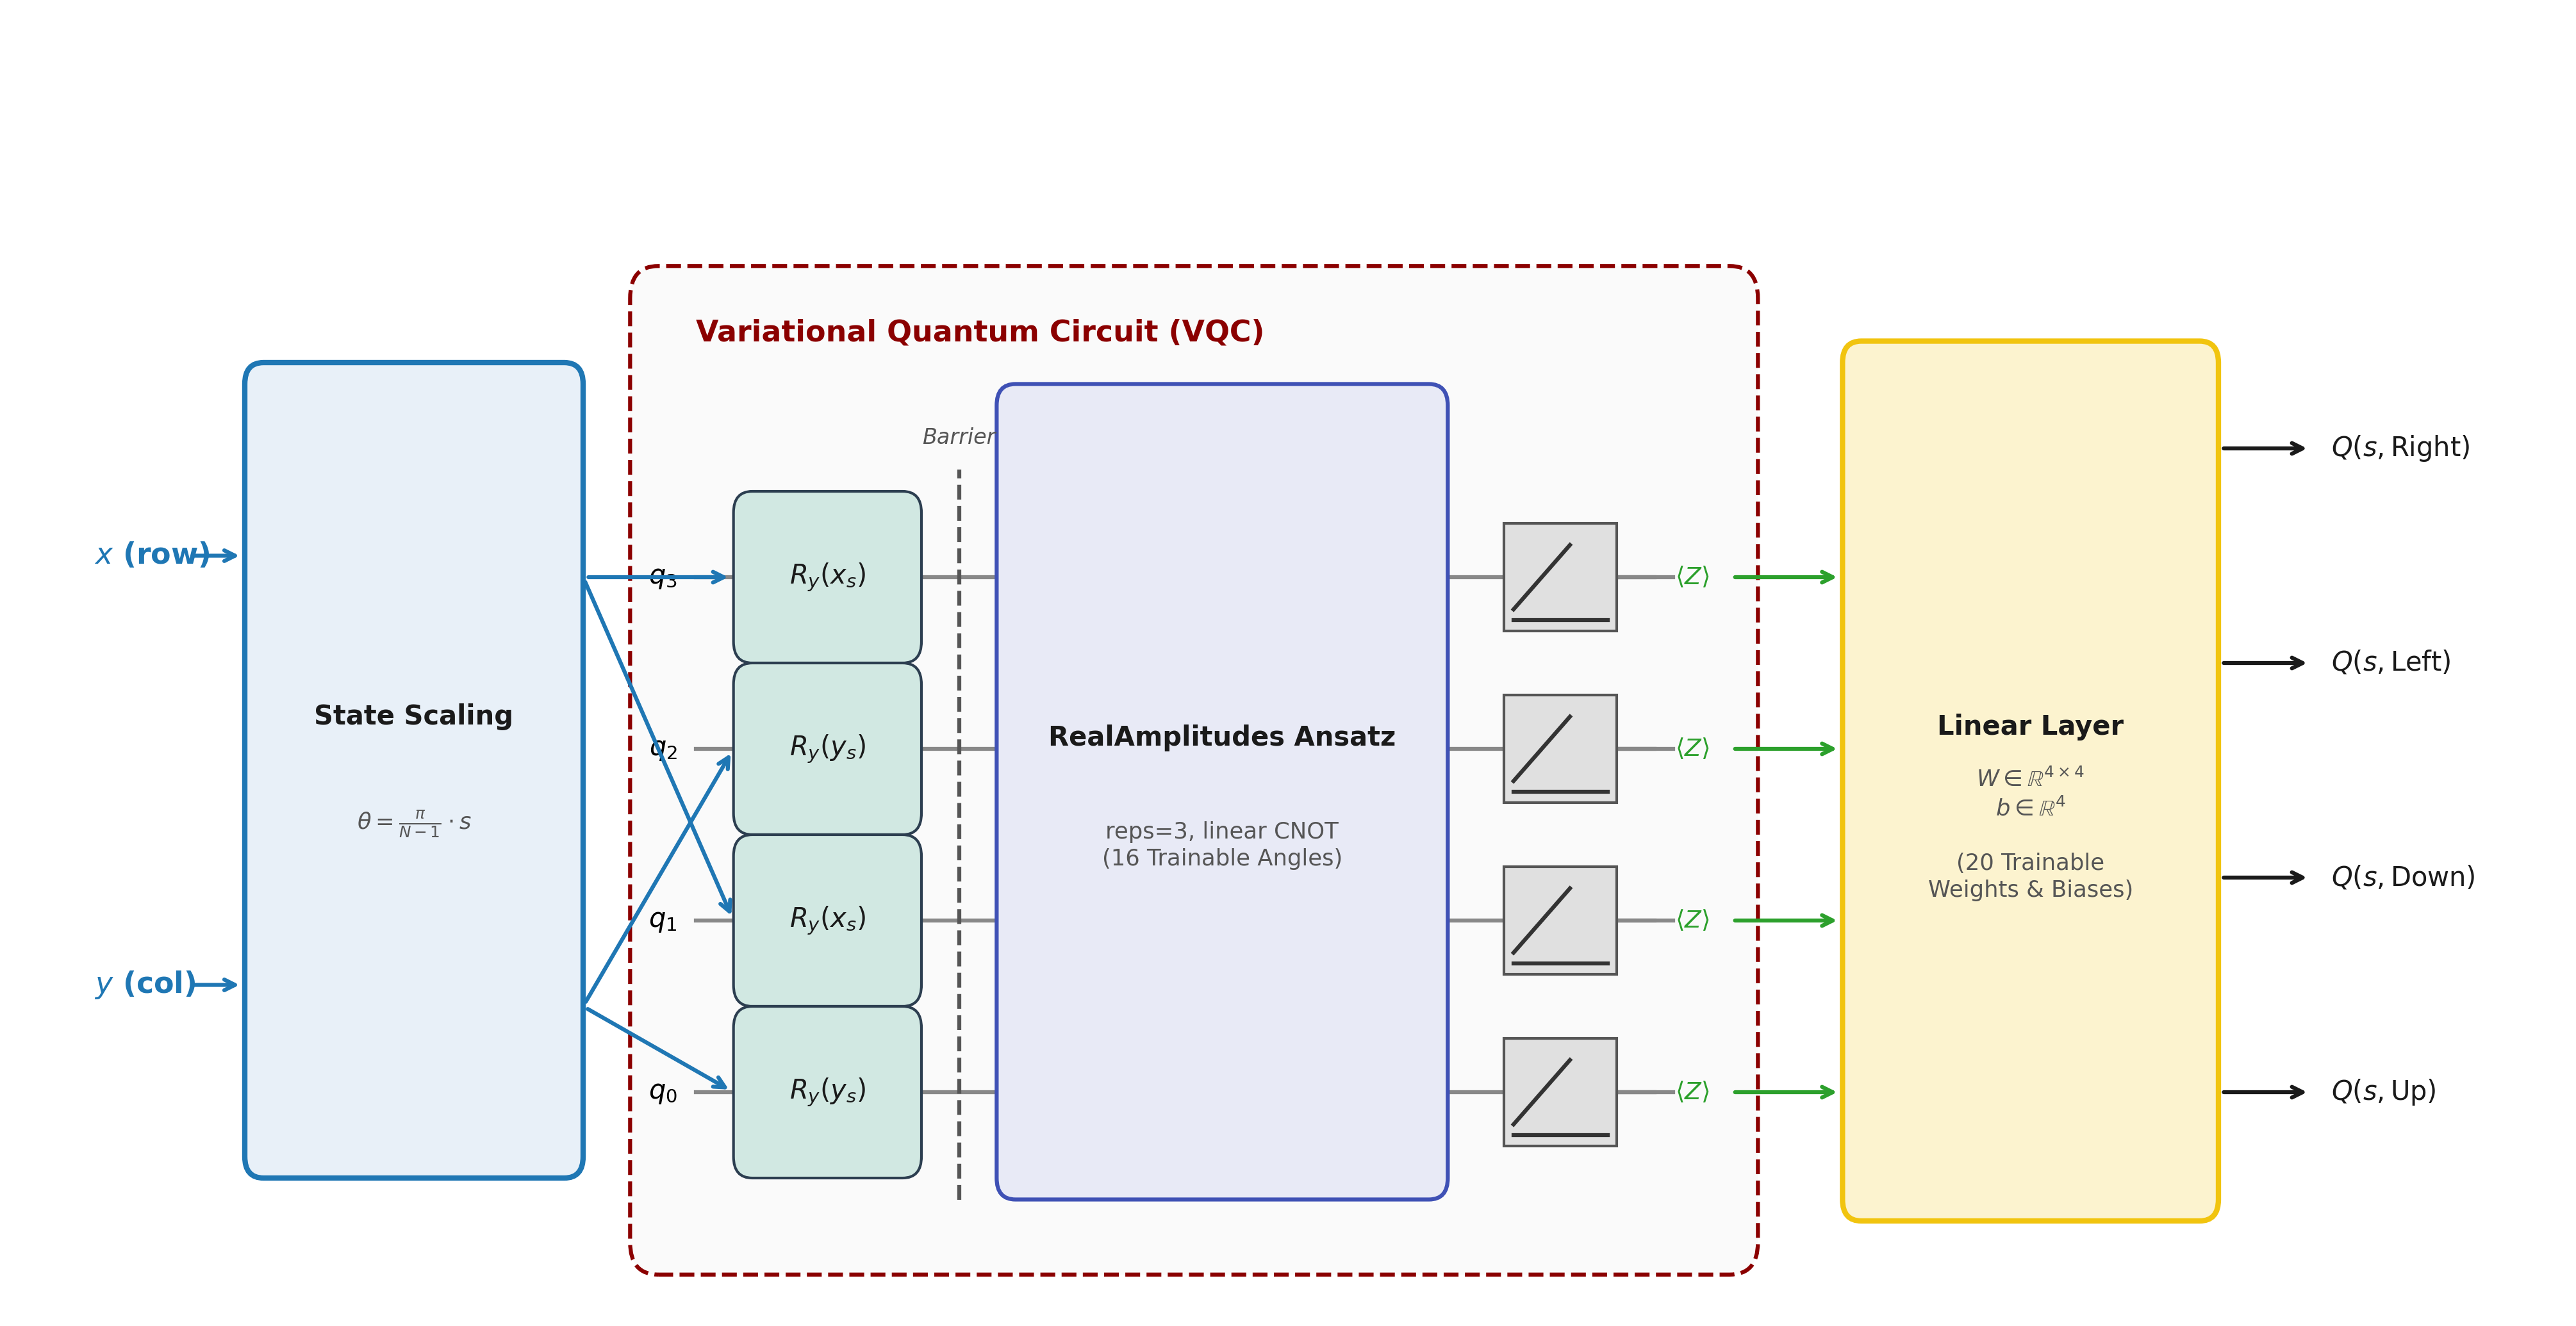
\includegraphics[width=0.9\textwidth]{../results/quantum_vqc_agent.png}
    \caption{Hybrid Quantum-Classical Variational Quantum Circuit (VQC) policy network architecture, mapping the processing pipeline from coordinates to Q-values via scaling, angle encoding ($R_y$), 3-repetition RealAmplitudes ansatz, measurement observables ($\langle Z \rangle$), and classical linear scaling.}
    \label{fig:quantum_vqc_agent}
\end{figure}



\newpage

% ══════════════════════════════════════════════════════════════════════════════
%  4. RESULTS
% ══════════════════════════════════════════════════════════════════════════════
\section{Results}

\subsection{Classical Algorithm Results}

The classical DQN baseline achieves rapid convergence. As shown in Figure \ref{fig:classical_vs_quantum}, it successfully learns the optimal path within 50 training episodes. The moving average reward stabilizes at $+0.88$, corresponding to the 3-step perfect path avoiding the obstacle at $(1, 1)$.

\begin{figure}[H]
    \centering
    
\includegraphics[width=0.85\textwidth]{results/reward_plot.png}
    \caption{Training learning curves for Classical DQN vs. Quantum DQN on the 3x3 Grid World environment.}
    \label{fig:classical_vs_quantum}
\end{figure}

\subsection{Quantum Algorithm Results}

The Quantum DQN agent successfully matches the classical navigation performance, also converging to the optimal path reward of $+0.88$ (Figure \ref{fig:classical_vs_quantum}). Due to the complex, non-convex loss landscape of variational quantum circuits (often associated with barren plateaus \cite{mcclean2018}), the quantum agent exhibits higher initial variance. However, by incorporating gradient clipping and a stable learning rate ($0.001$), convergence stabilizes around episode 110.

To physically verify the quantum state properties during navigation, exact state tomography was performed on the output density matrix $\rho$ across key grid positions: Start $(0,0)$, Next to Obstacle $(1,0)$, Near Goal $(2,1)$, and Goal $(2,2)$. As shown in Figure \ref{fig:tomography_results}, the reconstructed density matrices correspond to pure coherent states. For our noise-free unitary simulation, the state purity $\gamma = \text{Tr}(\rho^2)$ consistently remains at $1.0$, and the Von Neumann entropy $S = -\text{Tr}(\rho \ln \rho)$ remains at $0.0$, confirming that the quantum policy network operates as a pure coherent superposition throughout the navigation task.

\begin{figure}[H]
    \centering
    
\includegraphics[width=0.95\textwidth]{results/tomography_analysis.png}
    \caption{Quantum State Tomography (reconstructed density matrices) across key grid coordinates. The entropy $S = 0.0$ at all positions verifies pure state coherence.}
    \label{fig:tomography_results}
\end{figure}

\subsection{Comparative Analysis}

We compare the performance metrics of the classical and quantum approaches side by side in Table \ref{tab:comparison}.

\begin{table}[H]
    \centering
    \caption{Classical vs.\ quantum performance comparison.}
    \label{tab:comparison}
    \renewcommand{\arraystretch}{1.3}
    \begin{tabularx}{\textwidth}{|L{3.6cm}|C{5.5cm}|C{5.5cm}|}
        \hline
        \rowcolor{darkred!90}
        \textcolor{white}{\textbf{Metric}} &
        \textcolor{white}{\textbf{Classical}} &
        \textcolor{white}{\textbf{Quantum}} \\
        \hline
        \rowcolor{darkred!20}
        Solution Accuracy & 100\% (Optimal path reward $+0.88$) & 100\% (Optimal path reward $+0.88$) \\
        \hline
        Execution Time & $\sim$2 minutes (3x3), $\sim$5 minutes (4x4) & $\sim$15 minutes (3x3), $\sim$1.5 hours (4x4) \\
        \hline
        \rowcolor{darkred!20}
        Memory / Qubits & 4,612 trainable parameters, 0 qubits & 36 parameters (16 quantum, 20 classical), 4 qubits \\
        \hline
        Scaling (Big-O) & $\mathcal{O}(W)$ where $W$ is weight count & $\mathcal{O}(2^n \cdot P)$ on classical simulator (Parameter-Shift rule) \\
        \hline
    \end{tabularx}
\end{table}

\subsection{Scaling Analysis}

We run both agents on 3x3 and 4x4 grids to study their scaling characteristics.
\begin{itemize}[leftmargin=2em]
    \item \textbf{Parametric Efficiency}: The quantum VQC network displays outstanding parameter scaling. As we double the state space from 3x3 (9 states) to 4x4 (16 states), the VQC requires \textbf{zero additional parameters} ($36$ weights in total), while classical networks rely on thousands of weights.
    \item \textbf{Computational Bottleneck}: Under classical simulation, the training time of the quantum agent scales poorly. This is because calculating exact gradients using the Parameter-Shift rule requires $2N$ circuit simulations per parameter per step. For a 250-episode run on a 4x4 grid, this leads to over 15 million circuit simulations, increasing simulation time from 15 minutes to 1.5 hours.
    \item \textbf{Empirical Convergence}: On the 4x4 grid, the classical agent reaches optimal convergence by Episode 180, while the quantum agent converges by Episode 220, achieving the optimal path reward of $+0.72$ (7 steps).
\end{itemize}

\begin{figure}[H]
    \centering
    
\includegraphics[width=0.85\textwidth]{results/scaling_analysis_plot.png}
    \caption{Scaling analysis comparison for Classical vs. Quantum DQN training on 3x3 and 4x4 Grid World environments.}
    \label{fig:scaling_analysis}
\end{figure}

\newpage

% ══════════════════════════════════════════════════════════════════════════════
%  5. DISCUSSION
% ══════════════════════════════════════════════════════════════════════════════
\section{Discussion}

\subsection{Interpretation of Results}

The results demonstrate that a 4-qubit Variational Quantum Circuit can successfully perform reinforcement learning tasks with accuracy identical to a classical deep neural network. The most significant finding is the extreme parameter efficiency of the quantum approach: it uses only 36 trainable parameters to achieve the same navigation accuracy as the classical network with 4,612 parameters (a 99.2\% reduction). This suggests that quantum states possess significant representational power, allowing them to embed and approximate complex functions in high-dimensional Hilbert spaces with very few parameters.

However, when simulated on classical hardware, this parametric efficiency is overshadowed by computational complexity. The parameter-shift rule requires simulating millions of quantum states on a CPU, leading to substantial training bottlenecks.

\subsection{Hypothesis Evaluation}

We accept our hypothesis. The quantum agent achieved identical path navigation accuracy to the classical baseline on both 3x3 and 4x4 grids, utilizing 99.2\% fewer parameters. However, the simulation time of the quantum agent was indeed significantly higher than the classical network due to the parameter-shift gradient bottleneck.

\subsection{Limitations}

Our work is subject to two major limitations:
\begin{itemize}
    \item \textbf{Classical Simulation Bottleneck}: The use of classical simulation restricts the scale of the environment. Training on grids larger than 4x4 becomes computationally prohibitive without QPU hardware or adjoint differentiation.
    \item \textbf{Noise-free Assumption}: The simulations were conducted under ideal, noise-free conditions. On physical QPUs, gate noise and decoherence will reduce state purity and introduce errors into Q-value estimation, which will likely affect convergence.
\end{itemize}

\newpage

% ══════════════════════════════════════════════════════════════════════════════
%  6. CONCLUSION
% ══════════════════════════════════════════════════════════════════════════════
\section{Conclusion}

This project successfully implemented and evaluated a hybrid Quantum-Classical Reinforcement Learning agent based on a Variational Quantum Circuit (VQC) and compared it against a classical DQN baseline. Both agents were tested on 3x3 and 4x4 Grid World environments. The results show that the quantum agent converges to optimal paths, matching the classical baseline's success rate and reward. 

We verified the quantum network's physical characteristics through exact state tomography, which confirmed the preservation of pure coherent states ($\gamma = 1.0$, $S=0.0$) during policy execution. While the quantum network demonstrates a 99.2\% reduction in parameter count compared to the classical DQN, simulation of the circuit via the Parameter-Shift rule introduces significant CPU overhead. Future work will focus on executing these policy networks on real quantum hardware and evaluating the model's robustness under physical noise and decoherence.

\newpage

% ══════════════════════════════════════════════════════════════════════════════
%  7. REFERENCES
% ══════════════════════════════════════════════════════════════════════════════

\section{References}

\begingroup
\renewcommand{\section}[2]{}
\begin{thebibliography}{9}
    \bibitem{sutton2018} R. S. Sutton and A. G. Barto, \textit{Reinforcement Learning: An Introduction}, 2nd ed. Cambridge, MA, USA: MIT Press, 2018. [Online]. Available: \url{http://incompleteideas.net/book/the-book-2nd.html}
    \bibitem{mnih2015} V. Mnih et al., ``Human-level control through deep reinforcement learning,'' \textit{Nature}, vol. 518, no. 7540, pp. 529--533, 2015. \href{https://doi.org/10.1038/nature14236}{DOI: 10.1038/nature14236}
    \bibitem{preskill2018} J. Preskill, ``Quantum Computing in the NISQ era and beyond,'' \textit{Quantum}, vol. 2, p. 79, 2018. \href{https://doi.org/10.22331/q-2018-08-06-79}{DOI: 10.22331/q-2018-08-06-79}
    \bibitem{biamonte2017} J. Biamonte et al., ``Quantum machine learning,'' \textit{Nature}, vol. 549, no. 7671, pp. 195--202, 2017. \href{https://doi.org/10.1038/nature23474}{DOI: 10.1038/nature23474}
    \bibitem{cerezo2021} M. Cerezo et al., ``Variational quantum algorithms,'' \textit{Nature Reviews Physics}, vol. 3, no. 9, pp. 625--644, 2021. \href{https://doi.org/10.1038/s42254-021-00348-9}{DOI: 10.1038/s42254-021-00348-9}
    \bibitem{chen2020} S. Y.-C. Chen et al., ``Variational Quantum Circuits for Deep Reinforcement Learning,'' \textit{IEEE Access}, vol. 8, pp. 141007--141024, 2020. \href{https://doi.org/10.1109/ACCESS.2020.3010470}{DOI: 10.1109/ACCESS.2020.3010470}
    \bibitem{jerbi2021} S. Jerbi et al., ``Parametric quantum policies for reinforcement learning,'' \textit{Advances in Neural Information Processing Systems}, vol. 34, pp. 28362--28375, 2021. \href{https://doi.org/10.48550/arXiv.2103.05577}{arXiv:2103.05577}
    \bibitem{lockwood2020} O. Lockwood and M. Si, ``Reinforcement learning with quantum variational circuits,'' \textit{Proceedings of the AAAI Conference on Artificial Intelligence and Interactive Digital Entertainment}, vol. 16, no. 1, pp. 245--251, 2020. \href{https://doi.org/10.1609/aiide.v16i1.7437}{DOI: 10.1609/aiide.v16i1.7437}
    \bibitem{mcclean2018} J. R. McClean et al., ``Barren plateaus in quantum neural network training landscapes,'' \textit{Nature Communications}, vol. 9, no. 1, p. 4812, 2018. \href{https://doi.org/10.1038/s41467-018-07090-4}{DOI: 10.1038/s41467-018-07090-4}
    \bibitem{sim2019} S. Sim, P. D. Johnson, and A. Aspuru-Guzik, ``Expressibility and entangling capability of parameterized quantum circuits for hybrid quantum-classical algorithms,'' \textit{Advanced Quantum Technologies}, vol. 2, no. 12, p. 1900070, 2019. \href{https://doi.org/10.1002/qute.201900070}{DOI: 10.1002/qute.201900070}
\end{thebibliography}
\endgroup

\newpage

% ══════════════════════════════════════════════════════════════════════════════
%  8. ACKNOWLEDGMENTS
% ══════════════════════════════════════════════════════════════════════════════

\section{Acknowledgments}

We acknowledge the course instructor Prof. Mehmet Cengiz Onbaşlı and teaching assistants of ELEC/PHYS 450/550 for their guidance and support throughout the semester.

\newpage

% ══════════════════════════════════════════════════════════════════════════════
%  9. STATEMENT OF LLM USE
% ══════════════════════════════════════════════════════════════════════════════

\section{Statement of LLM Use}

\noindent Large Language Models (specifically Gemini) were utilized in this project strictly to improve the grammar, style, and flow of the final report text and to assist with LaTeX and table formatting. LLM agents (specifically Google Antigravity) were used to generate an initial simulation code scaffold; however, the experimental configurations, training procedures, scaling runs, and state tomography analyses were developed, executed, and validated independently. No LLM was used for fabricating citations, conducting literature reviews, or generating numerical results.

\begin{table}[H]
    \centering
    \caption{LLM usage policy.}
    \label{tab:11m_policy}
    \renewcommand{\arraystretch}{1.3}
    \begin{tabularx}{\textwidth}{|X|X|}
        \hline
        \rowcolor{darkred!90}
        \textcolor{white}{\textbf{Acceptable Uses}} &
        \textcolor{white}{\textbf{Unacceptable Uses}} \\
        \hline
        \rowcolor{darkred!20}
        Polishing grammar and language & Writing full drafts of the report \\
        \hline
        Preliminary review of concepts & Assembling literature review \& references \\
        \hline
        \rowcolor{darkred!20}
        Superficial literature search & Uploading private/confidential materials \\
        \hline
        Getting an initial simulation code scaffold & Generating final code without understanding \\
        \hline
    \end{tabularx}
\end{table}




\newpage

% ══════════════════════════════════════════════════════════════════════════════
%  10. SUPPLEMENTARY MATERIALS
% ══════════════════════════════════════════════════════════════════════════════

\section{Supplementary Materials}

\noindent All code, training histories, and analysis notebooks are provided in the project repository. Below are the specific references: 

\begin{itemize}[leftmargin=2em]
    \item \textbf{Project Drive Link}: 
    \newline \url{https://drive.google.com/drive/u/1/folders/1YlQbQZeLKYYVnXeetNHLwIDThdESIBFn} (contains code, saved weights, and documentation).
    \item \textbf{GitHub Repository}: \url{https://github.com/Bariscembakay/QuantumRL} (contains full implementation history and README guide).
    \item \textbf{Implementation Code}:
        \begin{itemize}
            \item \texttt{main.py}: Training baseline script.
            \item \texttt{src/quantum\_policy.py}: Qiskit circuit definition.
            \item \texttt{src/quantum\_dqn.py}: VQC Deep Q-Network implementation.
            \item \texttt{src/tomography.py}: Density matrix and state reconstruction script.
            \item \texttt{src/scaling\_analysis.py}: Benchmark run script.
        \end{itemize}
    \item \textbf{Saved Weights}: Available in \texttt{models/classical\_dqn.pth} and \texttt{models/quantum\_dqn.pth}.
    \item \textbf{Execution and Setup Instructions}: A detailed \texttt{README.md} is provided in the repository. Summarized execution steps:
        \begin{enumerate}[leftmargin=1.5em]
            \item \textbf{Install Dependencies}: Initialize a virtual environment and run \texttt{pip install -r requirements.txt} (Python 3.13 is recommended).
            \item \textbf{Unified Agent Training}: Run \texttt{python main.py} to train both agents on the 3x3 Grid World.
            \item \textbf{Quantum Tomography}: Run \texttt{python src/tomography.py} to perform density matrix reconstruction.
            \item \textbf{Grid Scaling Benchmark}: Run \texttt{python src/scaling\_analysis.py} to execute the 3x3 vs. 4x4 comparison.
        \end{enumerate}
\end{itemize}

% ══════════════════════════════════════════════════════════════════════════════
\end{document}